\section{Översikt av system}
Plattformen består av sammanlagt fyra enheter. En PC-enhet, en huvudenhet, en sensorenhet och en styrenhet. \\
PC-enheten är framförallt ett användargränssnitt som gör det enkelt för användaren att styra roboten och robotarmen men fungerar också som ett debugverktyg där användaren kan se robotens status och debuginformation. Huvudenheten står för huvuddelen av alla beräkningar roboten behöver göra så som regleringsalgoritm för linjeföljaren och koordinatkonvertering för armen. Sensorenheten innehåller den funktionalitet som krävs för att driva alla systemets sensorer och styrenheten innehåller den funktionalitet som krävs för att köra motorer och servon.

\begin{figure}[h]
\center
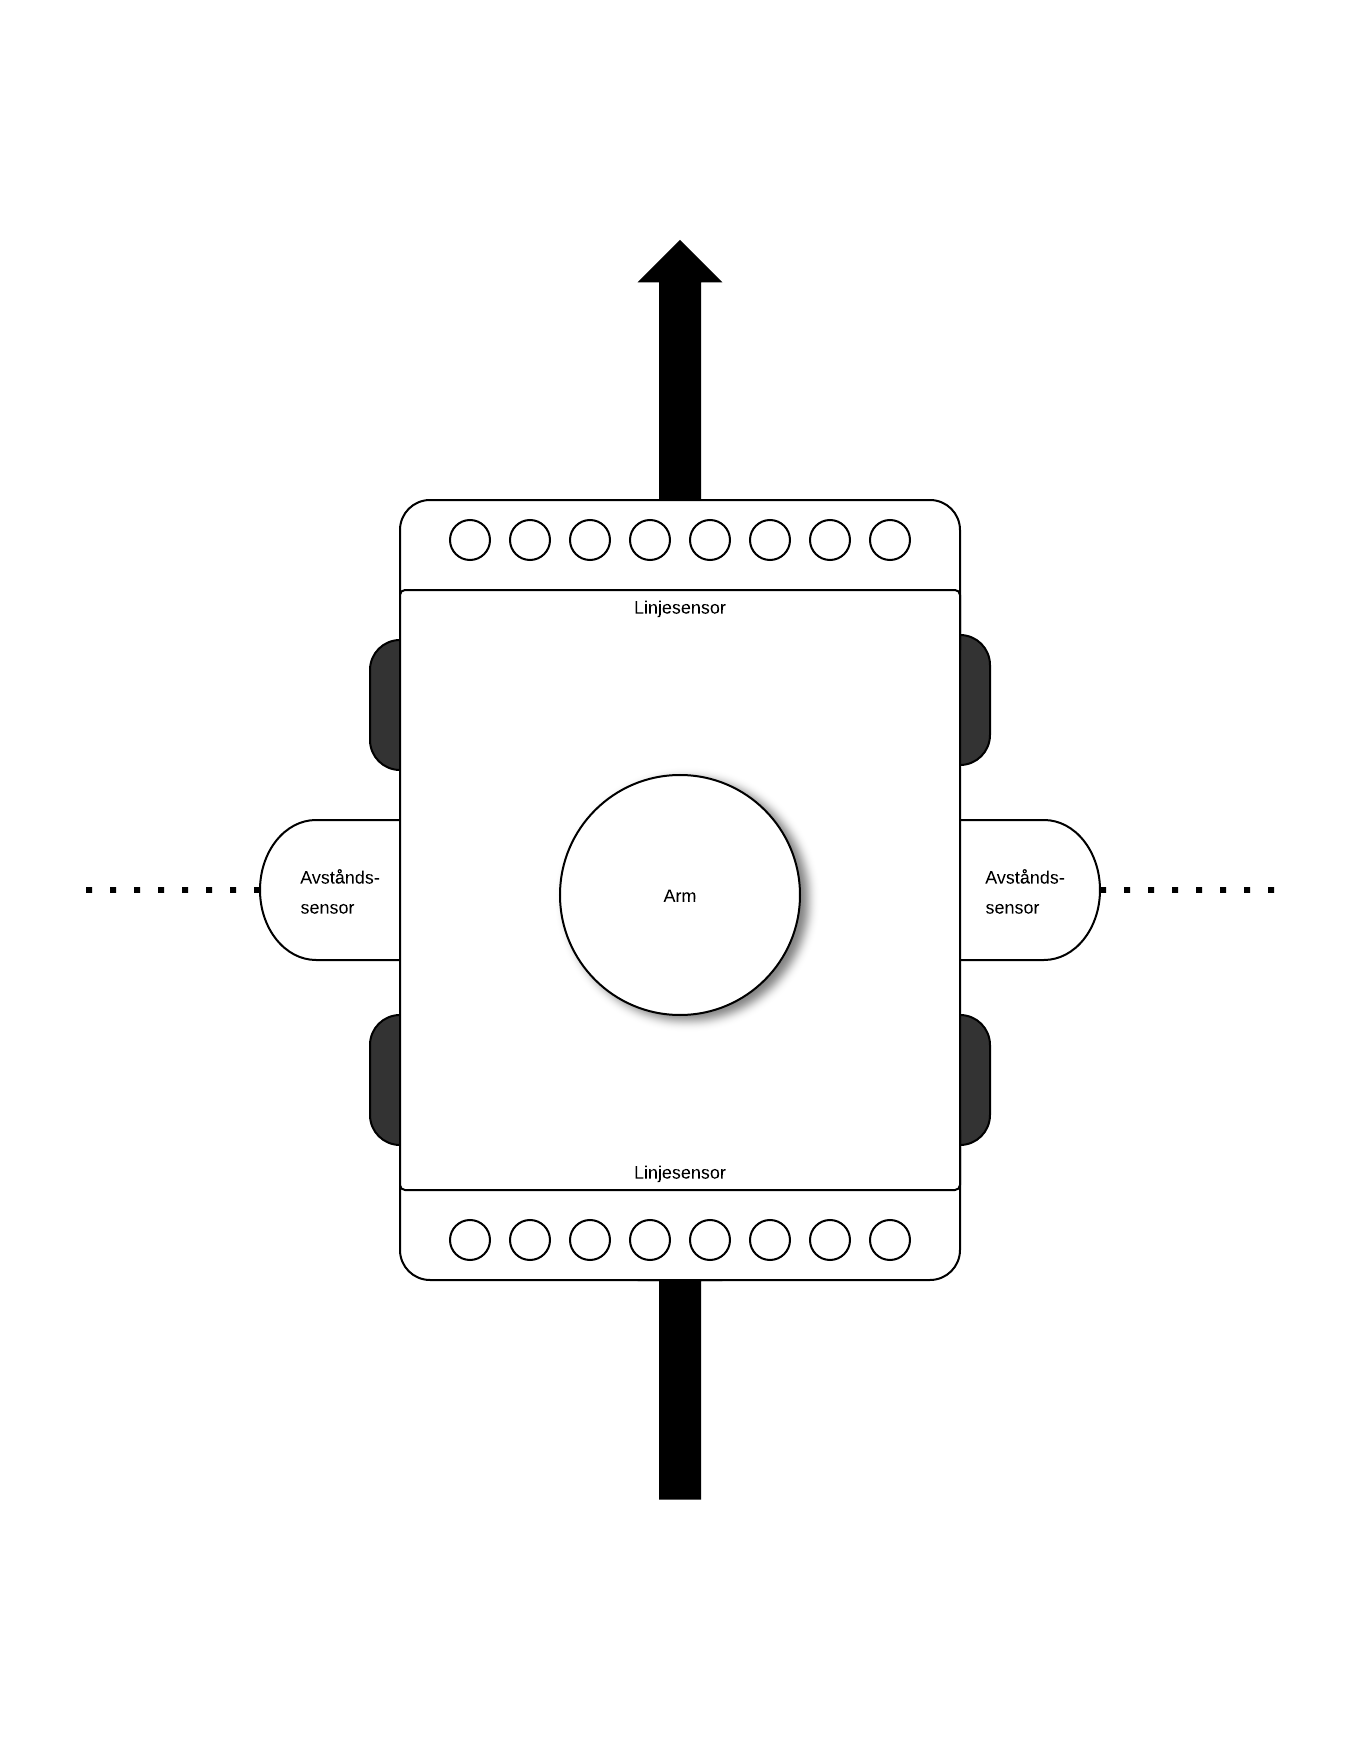
\includegraphics[scale=0.32]{robot}
\caption{Robot sedd ovanifrån. \todo{Rita om}} \label{designspec:robot}
\end{figure}

\subsection{Kommunikationskanaler}
I det fall att roboten arbetar i manuellt läge, skickar PC-enheten kommandon till huvudenheten över Bluetooth. I annat fall arbetar roboten autonomt och PC-enheten skickar endast förfrågningar angående robotens status. Huvudenheten skickar kommandon till sensorenheten och styrenheten över två SPI-bussar.

\begin{figure}[h]
\center
\scalebox{0.6}{% Graphic for TeX using PGF
% Title: /home/hannes/GitHub/TSEA29/dokumentation/designspecifikation/FLOW1.dia
% Creator: Dia v0.97.2
% CreationDate: Thu Oct  9 16:44:50 2014
% For: hannes
% \usepackage{tikz}
% The following commands are not supported in PSTricks at present
% We define them conditionally, so when they are implemented,
% this pgf file will use them.
\ifx\du\undefined
  \newlength{\du}
\fi
\setlength{\du}{15\unitlength}
\begin{tikzpicture}
\pgftransformxscale{1.000000}
\pgftransformyscale{-1.000000}
\definecolor{dialinecolor}{rgb}{0.000000, 0.000000, 0.000000}
\pgfsetstrokecolor{dialinecolor}
\definecolor{dialinecolor}{rgb}{1.000000, 1.000000, 1.000000}
\pgfsetfillcolor{dialinecolor}
\definecolor{dialinecolor}{rgb}{1.000000, 1.000000, 1.000000}
\pgfsetfillcolor{dialinecolor}
\fill (2.704150\du,11.806300\du)--(2.704150\du,18.306300\du)--(12.454150\du,18.306300\du)--(12.454150\du,11.806300\du)--cycle;
\pgfsetlinewidth{0.100000\du}
\pgfsetdash{}{0pt}
\pgfsetdash{}{0pt}
\pgfsetmiterjoin
\definecolor{dialinecolor}{rgb}{0.000000, 0.000000, 0.000000}
\pgfsetstrokecolor{dialinecolor}
\draw (2.704150\du,11.806300\du)--(2.704150\du,18.306300\du)--(12.454150\du,18.306300\du)--(12.454150\du,11.806300\du)--cycle;
% setfont left to latex
\definecolor{dialinecolor}{rgb}{0.000000, 0.000000, 0.000000}
\pgfsetstrokecolor{dialinecolor}
\node at (7.579150\du,15.251300\du){HUVUDENHET};
\definecolor{dialinecolor}{rgb}{1.000000, 1.000000, 1.000000}
\pgfsetfillcolor{dialinecolor}
\fill (-6.345850\du,13.456300\du)--(-6.345850\du,16.806300\du)--(-1.645850\du,16.806300\du)--(-1.645850\du,13.456300\du)--cycle;
\pgfsetlinewidth{0.100000\du}
\pgfsetdash{}{0pt}
\pgfsetdash{}{0pt}
\pgfsetmiterjoin
\definecolor{dialinecolor}{rgb}{0.000000, 0.000000, 0.000000}
\pgfsetstrokecolor{dialinecolor}
\draw (-6.345850\du,13.456300\du)--(-6.345850\du,16.806300\du)--(-1.645850\du,16.806300\du)--(-1.645850\du,13.456300\du)--cycle;
% setfont left to latex
\definecolor{dialinecolor}{rgb}{0.000000, 0.000000, 0.000000}
\pgfsetstrokecolor{dialinecolor}
\node at (-3.995850\du,15.326300\du){SPI};
\definecolor{dialinecolor}{rgb}{1.000000, 1.000000, 1.000000}
\pgfsetfillcolor{dialinecolor}
\fill (16.254200\du,13.256300\du)--(16.254200\du,16.756300\du)--(21.104200\du,16.756300\du)--(21.104200\du,13.256300\du)--cycle;
\pgfsetlinewidth{0.100000\du}
\pgfsetdash{}{0pt}
\pgfsetdash{}{0pt}
\pgfsetmiterjoin
\definecolor{dialinecolor}{rgb}{0.000000, 0.000000, 0.000000}
\pgfsetstrokecolor{dialinecolor}
\draw (16.254200\du,13.256300\du)--(16.254200\du,16.756300\du)--(21.104200\du,16.756300\du)--(21.104200\du,13.256300\du)--cycle;
% setfont left to latex
\definecolor{dialinecolor}{rgb}{0.000000, 0.000000, 0.000000}
\pgfsetstrokecolor{dialinecolor}
\node at (18.679200\du,15.201300\du){SPI};
\pgfsetlinewidth{0.100000\du}
\pgfsetdash{}{0pt}
\pgfsetdash{}{0pt}
\pgfsetbuttcap
{
\definecolor{dialinecolor}{rgb}{0.000000, 0.000000, 0.000000}
\pgfsetfillcolor{dialinecolor}
% was here!!!
\pgfsetarrowsstart{to}
\pgfsetarrowsend{to}
\definecolor{dialinecolor}{rgb}{0.000000, 0.000000, 0.000000}
\pgfsetstrokecolor{dialinecolor}
\draw (-1.595931\du,15.115750\du)--(2.654971\du,15.088206\du);
}
\pgfsetlinewidth{0.100000\du}
\pgfsetdash{}{0pt}
\pgfsetdash{}{0pt}
\pgfsetbuttcap
{
\definecolor{dialinecolor}{rgb}{0.000000, 0.000000, 0.000000}
\pgfsetfillcolor{dialinecolor}
% was here!!!
\pgfsetarrowsstart{to}
\pgfsetarrowsend{to}
\definecolor{dialinecolor}{rgb}{0.000000, 0.000000, 0.000000}
\pgfsetstrokecolor{dialinecolor}
\draw (12.503849\du,15.034117\du)--(16.204317\du,15.017448\du);
}
\definecolor{dialinecolor}{rgb}{1.000000, 1.000000, 1.000000}
\pgfsetfillcolor{dialinecolor}
\fill (-8.145850\du,19.856300\du)--(-8.145850\du,25.956300\du)--(0.354150\du,25.956300\du)--(0.354150\du,19.856300\du)--cycle;
\pgfsetlinewidth{0.100000\du}
\pgfsetdash{}{0pt}
\pgfsetdash{}{0pt}
\pgfsetmiterjoin
\definecolor{dialinecolor}{rgb}{0.000000, 0.000000, 0.000000}
\pgfsetstrokecolor{dialinecolor}
\draw (-8.145850\du,19.856300\du)--(-8.145850\du,25.956300\du)--(0.354150\du,25.956300\du)--(0.354150\du,19.856300\du)--cycle;
% setfont left to latex
\definecolor{dialinecolor}{rgb}{0.000000, 0.000000, 0.000000}
\pgfsetstrokecolor{dialinecolor}
\node at (-3.895850\du,23.101300\du){STYRENHET};
\definecolor{dialinecolor}{rgb}{1.000000, 1.000000, 1.000000}
\pgfsetfillcolor{dialinecolor}
\fill (14.404200\du,19.406300\du)--(14.404200\du,25.606300\du)--(22.904200\du,25.606300\du)--(22.904200\du,19.406300\du)--cycle;
\pgfsetlinewidth{0.100000\du}
\pgfsetdash{}{0pt}
\pgfsetdash{}{0pt}
\pgfsetmiterjoin
\definecolor{dialinecolor}{rgb}{0.000000, 0.000000, 0.000000}
\pgfsetstrokecolor{dialinecolor}
\draw (14.404200\du,19.406300\du)--(14.404200\du,25.606300\du)--(22.904200\du,25.606300\du)--(22.904200\du,19.406300\du)--cycle;
% setfont left to latex
\definecolor{dialinecolor}{rgb}{0.000000, 0.000000, 0.000000}
\pgfsetstrokecolor{dialinecolor}
\node at (18.654200\du,22.701300\du){SENSORENHET};
\pgfsetlinewidth{0.100000\du}
\pgfsetdash{}{0pt}
\pgfsetdash{}{0pt}
\pgfsetbuttcap
{
\definecolor{dialinecolor}{rgb}{0.000000, 0.000000, 0.000000}
\pgfsetfillcolor{dialinecolor}
% was here!!!
\pgfsetarrowsstart{to}
\pgfsetarrowsend{to}
\definecolor{dialinecolor}{rgb}{0.000000, 0.000000, 0.000000}
\pgfsetstrokecolor{dialinecolor}
\draw (-3.973670\du,16.855809\du)--(-3.935724\du,19.806076\du);
}
\pgfsetlinewidth{0.100000\du}
\pgfsetdash{}{0pt}
\pgfsetdash{}{0pt}
\pgfsetbuttcap
{
\definecolor{dialinecolor}{rgb}{0.000000, 0.000000, 0.000000}
\pgfsetfillcolor{dialinecolor}
% was here!!!
\pgfsetarrowsstart{to}
\pgfsetarrowsend{to}
\definecolor{dialinecolor}{rgb}{0.000000, 0.000000, 0.000000}
\pgfsetstrokecolor{dialinecolor}
\draw (18.673199\du,16.806685\du)--(18.664700\du,19.356428\du);
}
\definecolor{dialinecolor}{rgb}{1.000000, 1.000000, 1.000000}
\pgfsetfillcolor{dialinecolor}
\fill (5.729150\du,6.781310\du)--(5.729150\du,9.481310\du)--(9.379150\du,9.481310\du)--(9.379150\du,6.781310\du)--cycle;
\pgfsetlinewidth{0.100000\du}
\pgfsetdash{}{0pt}
\pgfsetdash{}{0pt}
\pgfsetmiterjoin
\definecolor{dialinecolor}{rgb}{0.000000, 0.000000, 0.000000}
\pgfsetstrokecolor{dialinecolor}
\draw (5.729150\du,6.781310\du)--(5.729150\du,9.481310\du)--(9.379150\du,9.481310\du)--(9.379150\du,6.781310\du)--cycle;
% setfont left to latex
\definecolor{dialinecolor}{rgb}{0.000000, 0.000000, 0.000000}
\pgfsetstrokecolor{dialinecolor}
\node at (7.554150\du,7.926310\du){BT};
% setfont left to latex
\definecolor{dialinecolor}{rgb}{0.000000, 0.000000, 0.000000}
\pgfsetstrokecolor{dialinecolor}
\node at (7.554150\du,8.726310\du){USB};
\pgfsetlinewidth{0.100000\du}
\pgfsetdash{}{0pt}
\pgfsetdash{}{0pt}
\pgfsetbuttcap
{
\definecolor{dialinecolor}{rgb}{0.000000, 0.000000, 0.000000}
\pgfsetfillcolor{dialinecolor}
% was here!!!
\pgfsetarrowsstart{to}
\pgfsetarrowsend{to}
\definecolor{dialinecolor}{rgb}{0.000000, 0.000000, 0.000000}
\pgfsetstrokecolor{dialinecolor}
\draw (7.559205\du,9.531609\du)--(7.567334\du,11.783160\du);
}
\definecolor{dialinecolor}{rgb}{1.000000, 1.000000, 1.000000}
\pgfsetfillcolor{dialinecolor}
\fill (4.921370\du,-4.547630\du)--(4.921370\du,-1.269208\du)--(10.224661\du,-1.269208\du)--(10.224661\du,-4.547630\du)--cycle;
\pgfsetlinewidth{0.100000\du}
\pgfsetdash{}{0pt}
\pgfsetdash{}{0pt}
\pgfsetmiterjoin
\definecolor{dialinecolor}{rgb}{0.000000, 0.000000, 0.000000}
\pgfsetstrokecolor{dialinecolor}
\draw (4.921370\du,-4.547630\du)--(4.921370\du,-1.269208\du)--(10.224661\du,-1.269208\du)--(10.224661\du,-4.547630\du)--cycle;
% setfont left to latex
\definecolor{dialinecolor}{rgb}{0.000000, 0.000000, 0.000000}
\pgfsetstrokecolor{dialinecolor}
\node at (7.573016\du,-2.713419\du){PC};
\definecolor{dialinecolor}{rgb}{1.000000, 1.000000, 1.000000}
\pgfsetfillcolor{dialinecolor}
\fill (5.938090\du,1.451670\du)--(5.938090\du,4.151670\du)--(9.155420\du,4.151670\du)--(9.155420\du,1.451670\du)--cycle;
\pgfsetlinewidth{0.100000\du}
\pgfsetdash{}{0pt}
\pgfsetdash{}{0pt}
\pgfsetmiterjoin
\definecolor{dialinecolor}{rgb}{0.000000, 0.000000, 0.000000}
\pgfsetstrokecolor{dialinecolor}
\draw (5.938090\du,1.451670\du)--(5.938090\du,4.151670\du)--(9.155420\du,4.151670\du)--(9.155420\du,1.451670\du)--cycle;
% setfont left to latex
\definecolor{dialinecolor}{rgb}{0.000000, 0.000000, 0.000000}
\pgfsetstrokecolor{dialinecolor}
\node at (7.546755\du,2.596670\du){USB};
% setfont left to latex
\definecolor{dialinecolor}{rgb}{0.000000, 0.000000, 0.000000}
\pgfsetstrokecolor{dialinecolor}
\node at (7.546755\du,3.396670\du){BT};
\pgfsetlinewidth{0.100000\du}
\pgfsetdash{}{0pt}
\pgfsetdash{}{0pt}
\pgfsetbuttcap
{
\definecolor{dialinecolor}{rgb}{0.000000, 0.000000, 0.000000}
\pgfsetfillcolor{dialinecolor}
% was here!!!
\pgfsetarrowsstart{to}
\pgfsetarrowsend{to}
\definecolor{dialinecolor}{rgb}{0.000000, 0.000000, 0.000000}
\pgfsetstrokecolor{dialinecolor}
\draw (7.565258\du,-1.221601\du)--(7.553194\du,1.401681\du);
}
\pgfsetlinewidth{0.100000\du}
\pgfsetdash{{\pgflinewidth}{0.200000\du}}{0cm}
\pgfsetdash{{\pgflinewidth}{0.200000\du}}{0cm}
\pgfsetbuttcap
{
\definecolor{dialinecolor}{rgb}{0.000000, 0.000000, 0.000000}
\pgfsetfillcolor{dialinecolor}
% was here!!!
\pgfsetarrowsstart{to}
\pgfsetarrowsend{to}
\definecolor{dialinecolor}{rgb}{0.000000, 0.000000, 0.000000}
\pgfsetstrokecolor{dialinecolor}
\draw (7.548694\du,4.199139\du)--(7.552211\du,6.733841\du);
}
\end{tikzpicture}
}
\caption{Flödesschema över kommunikationskanalerna i systemet.}
\end{figure}

\subsection{Uppgraderbarhet}
Kommunikation mellan huvudmodulen och PC-enheten kommer att ske över bluetooth och kommer att användas för att sätta upp ett PAN. Över denna sätts en TCP/IP anslutning upp och data skickas över en Python-socket vilket leder till att bluetooth kan bytas ut mot till exempel WIFI, en ethernetkabel eller annan överföringskanal som tillåter tcp/ip.\newline
\newline
Kommunikationen mellan huvudmodulen och styrenheten samt sensormodulen sker över två I2C bussor över välspecificerade protokoll. Om det önskas kan sensormodulen coh styrmodulen bytas ut mot andra moduler så länge de använder samma protokoll. Styrenheten kommunicerar med servona över UART och använder Trossenrobotics egna protokoll vilket leder till att armen inte kan bytas ut mot någon annan.
